 % use the "wcp" class option for workshop and conference
 % proceedings
 %\documentclass[gray]{jmlr} % test grayscale version
 %\documentclass[tablecaption=bottom]{jmlr}% journal article
 \documentclass[tablecaption=bottom,nowcp]{jmlr}% W&CP article

 % The following packages will be automatically loaded:
 % amsmath, amssymb, natbib, graphicx, url, algorithm2e

 %\usepackage{rotating}% for sideways figures and tables
 %\usepackage{longtable}% for long tables

 % The booktabs package is used by this sample document
 % (it provides \toprule, \midrule and \bottomrule).
 % Remove the next line if you don't require it.
\usepackage{booktabs}
 % The siunitx package is used by this sample document
 % to align numbers in a column by their decimal point.
 % Remove the next line if you don't require it.
\usepackage[load-configurations=version-1]{siunitx} % newer version
 %\usepackage{siunitx}

 % Define an unnumbered theorem just for this sample document for
 % illustrative purposes:
\theorembodyfont{\upshape}
\theoremheaderfont{\scshape}
\theorempostheader{:}
\theoremsep{\newline}
\newtheorem*{note}{Note}

\jmlrproceedings{ML project}{ML project}

\title{Time Series forecasting with Temporal Fusion Transformers}

\author{\Name{Damir Khabibulin}\\
  \addr Higher School of Economics}


\begin{document}

\maketitle

% Keywords may be removed
%\begin{keywords}
%List of keywords
%\end{keywords}

\section{Introduction}
\label{sec:intro}

In this project I research interpretable model for multi-horizon time series forecasting based on temporal fusion transformers that was proposed in the article [1]. The model will be reproduced on PyTorch framework, then I will extend training data for model and will experiment with hyperparameters and model.

\section{Motivation}
\label{sec:mot}

Multi-horizon forecasting is the prediction for estimates across several steps in future. It has many real-world applications. Typically, models provide forecasts from “black-box” models, while Temporal Fusion Transformer combines high-performance multi-horizon forecasting with interpretable insights into temporal dynamics.

\section{Temporal Fusion Transformers}
\label{sec:tft}

If we take $I$ as unique entitles in a given time series dataset, in this project it is a different stock assets. Each entity $i$ is associated with a set of static covariates ${\vec{s}_i \in {\mathbb{R}}^{m_s}}$, as well as inputs ${\vec{X}_{i,t} \in {\mathbb{R}}^{m_x}}$ and scalar targets ${\vec{y}_{i,t} \in {\mathbb{R}}}$ as each time-step ${t \in [0,T_i]}$. Time-dependent input features are
subdivided into two categories ${\vec{X}_{i,t} \in [\vec{z}_{i,t}^T,\vec{x}_{i,t}^T]^T}$ - observed inputs
${\vec{z}_{i,t} \in {\mathbb{R}}^{(m_z)}}$ which can only be measured at each step and are unknown beforehand, and known inputs ${\vec{x}_{i,t} \in {\mathbb{R}}^{m_x}}$ which can be predetermined (e.g. the day-of-week at time t).
In many scenarios, the provision for prediction intervals can be useful for optimizing decisions and risk management by yielding an indication of likely best and worst-case values that the target can take. As such, we adopt quantile regression to our multi-horizon forecasting setting (e.g. outputting the 10th, 50th and 90th percentiles at each time step). Each quantile forecast takes the form:
\begin{equation}
\hat{y_i}(q,t,\tau) = f_q(\tau, y_{i,t-k:t}, \vec{z}_{i,t-k:t+\tau},\vec{s_i}),
\end{equation}
where $\hat{y}_{i,t+\tau}(q,t,\tau)$  is the predicted $q^{th}$ sample quantile of the $\tau$-step-ahead 
forecast at time $t$, and $f_q(.)$ is a prediction model.  In line with other direct methods, we simultaneously output forecasts for $\tau_max$ time steps - $\tau \in \{1,...,\tau_max\}$. We incorporate all past information within a finite look-back window $k$, using target and known inputs only up till and including the forecast start time $t$ (i.e. $y_{i,t-k:t}=\{y_{i,t-k},...,y_{i,t}\}$) and known inputs across the entire range (i.e. $\vec{x}_{i,t-k:t}=\{\vec{x}_{i,t-k},...,\vec{x}_{i,t},...,\vec{x}_{i,t+\tau}\}$)


\section{Model Architecture}
\label{sec:model}

\begin{figure}[htbp]
\floatconts
  {fig:nodes}
  {\caption{Model Architecture}}
  {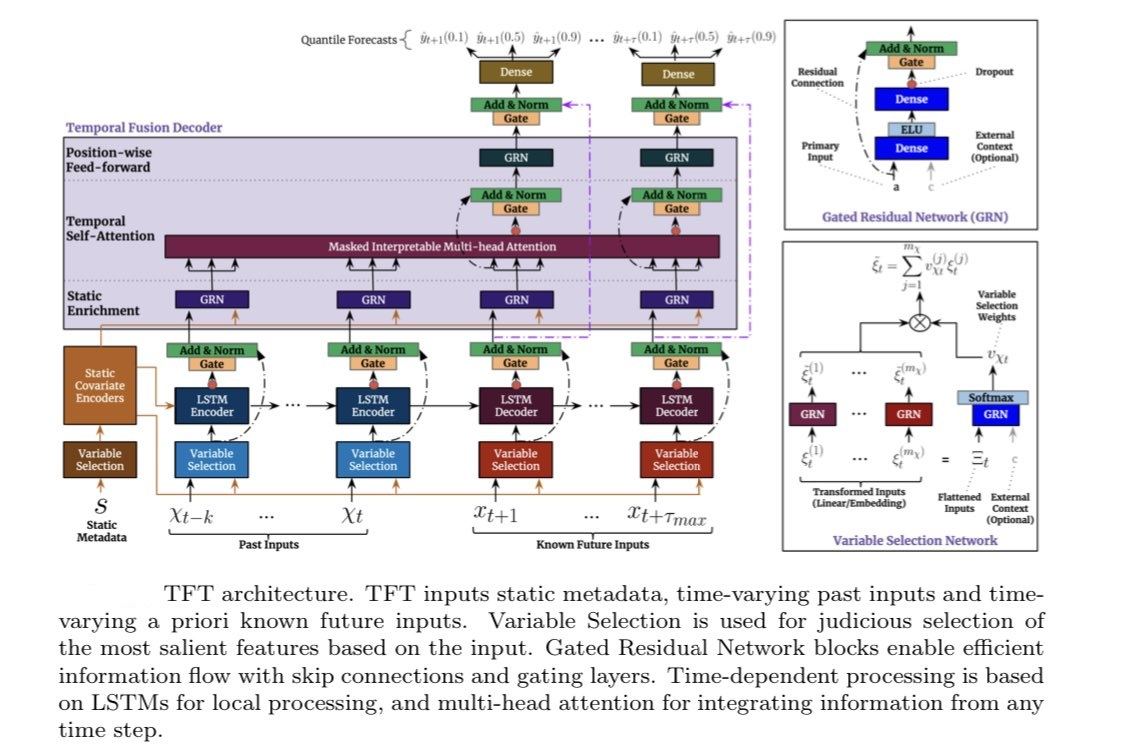
\includegraphics[width=1\linewidth]{1.jpg}}
\end{figure}

\begin{enumerate}
\item Gating mechanisms to skip over any unused components of the architecture, providing adaptive depth and network complexity to accommodate a wide range of datasets and scenarios.
\item Variable selection networks to select relevant input variables at each time step.
\item Static covariate encoders to integrate static features into the network, through encoding of context vectors to condition temporal dynamics.
\item Temporal processing to learn both long- and short-term temporal relationships from both observed and known time-varying inputs. A sequenceto-sequence layer is employed for local processing, whereas long-term dependencies are captured using a novel interpretable multi-head attention block.
\item Prediction intervals via quantile forecasts to determine the range of likely target values at each prediction horizon
\end{enumerate}

\section{Experiments}
\label{sec:exp}

\subsection{Volatility prediction}
\label{sec:vol}
In this experiment I used proposed dataset [2] that contains daily non-parametric measures of how volatility financial assets or indexes were in the past. Each day's volatility measure depends solely on financial data from that day. I have trained model on this dataset and checked perfomance.

\subsection{Change Softmax to SM-Taylor softmax}
\label{sec:smx}
Softmax function is a popular choice in deep learning classification tasks. Recently,
this function has found application in other operations as well, such as the attention mechanisms. In this project I replaced softmax with SM-Taylor softmax [3]. Then trained model and checked perfomance.

\subsection{Test on simple dataset}
\label{sec:smx}
I have generated three simple datasets and checked perfomance.

\section{Results}
\label{sec:res}
On a simple datasets that contain only known inputs and complex datasets which encompass the full range of possible inputs – we show that TFT achieves state-of-the-art forecasting performance.
\\Changing model in both cases came up to overfitting.
\\The code used for this project presents in this repository:
\\\url{https://github.com/damu4/tft-forecast}
\\Examples of predictions:
\begin{figure}[htbp]
\floatconts
  {fig:nodes}
  {\caption{Volatility predictions for asset "SPX"}}
  {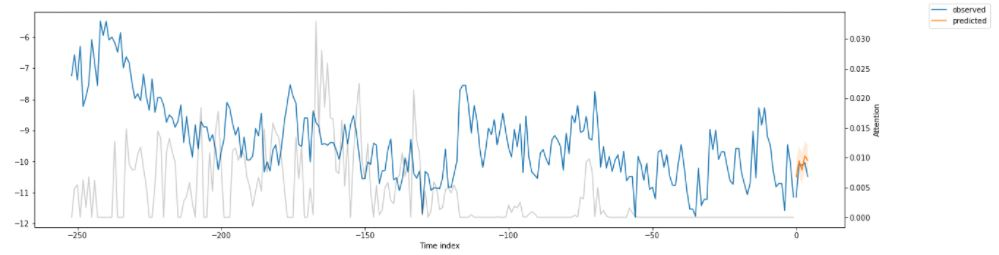
\includegraphics[width=1\linewidth]{spx.jpg}}
\end{figure}
\begin{figure}[htbp]
\floatconts
  {fig:nodes}
  {\caption{sin(x/2)}}
  {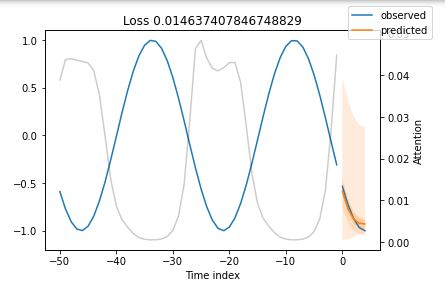
\includegraphics[width=0.5\linewidth]{s1.JPG}}
\end{figure}
\begin{figure}[htbp]
\floatconts
  {fig:nodes}
  {\caption{sin(x/8)}}
  {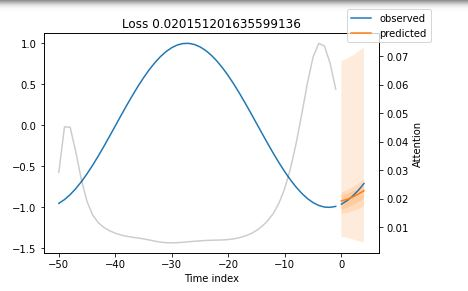
\includegraphics[width=0.5\linewidth]{s2.jpg}}
\end{figure}
\begin{figure}[htbp]
\floatconts
  {fig:nodes}
  {\caption{sin(x/4) with noise}}
  {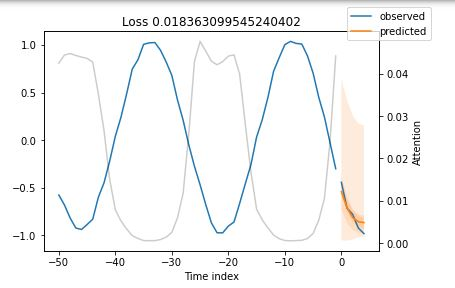
\includegraphics[width=0.5\linewidth]{s3.jpg}}
\end{figure}

\section{References}
\label{sec:ref}
[1] Bryan Lim, Sercan O. Arik, Nicolas Loeff, Tomas Pfister (2019). Temporal Fusion Transformers for Interpretable Multi-horizon Time Series Forecasting.\par
\noindent
[2] G. Heber, A. Lunde, N. Shephard, K. K. Sheppard, Oxford-man institute’s realized library (2009). \url{https://realized.oxford-man.ox.ac.uk}\par
\noindent
[3] Kunal Banerjee, Vishak Prasad C, Rishi Raj Gupta, Karthik Vyas, Anushree H, Biswajit Mishra. Exploring Alternatives to Softmax Function\par
\end{document}
